\section{Графоструктурное моделирование} 
Цель данной главы -- провести обзор литературы и программного обеспечения по теме графоструктурного моделирования и его прикладных приложений и представить описание развития графовых структур в виде последовательности обобщения одних графовых структур другими: графы $\to$ орграфы $\to$ гиперграфы $\to$ оргиперграфы $\to$ метаграфы $\to$ орметаграфы $\to$ гипергиперграфы $\to$ оргипергиперграфы $\to$ итерированные гиперграфы $\to$ ...

В конце главы формулируется цель выпускной квалификационной работы и ставятся соответсвующие задачи.

\subsection{Графовые структуры и их взаимосвязь}
Графовые структуры широко применяются в моделировании и управлении реальными объектами самой разнообразной природы. В последнее время графовые структуры получили существенное развитие: от обычных графов до итерированных гиперграфов, представляющих иерархические структуры высокого уровня абстракции. 

Для описания и анализа больших данных, в зависимости от предметной области и требуемых результатов, могут быть применены как различные подходы к моделированию, так и различные модели из одного кластера, присущего конкретному подходу. Графы являются наиболее популярными моделями графоструктурного подхода, это обусловлено прежде всего интуитивной геометрической интерпретацией и тем, что они являются простейшим типом графовых структур, имеющим широкий спектр прикладного применения. Хотя графы и покрывают значительную часть разнообразия задач дискретного моделирования, но обобщённые графовые структуры последнее время укрепляют свои позиции в задачах моделирования систем в различных областях, которые в принципе формально представимы графами, но слишком усложнены либо количественными показателями, что непосредственно сказывается на эффективности вычислений, либо структурой, которая в свою очередь может быть столь сложной, что её декомпозиция на бинарные отношения для моделирования на графах приведёт к невозможности анализа и интерпретации конечных результатов и трудностям целостного моделирования без потери системного эффекта, так называемых эмерджентных свойств. Хорошей иллюстрацией системы с эмерджентными свойствами может служить текст на естественном языке. Каждое предложение, как и слово, несёт в себе определённую информацию, предысторию, свойства, и только при рассмотрении текста как целостной системы возникает характерная ему уникальность, определённая структурой и информацией, в общем случае невыводимая из элементов его декомпозиции [1]. Необходимо заметить, под моделированием системы целостно понимается моделирование нескольких уровней абстракции этой системы в совокупности, что является, в некотором смысле, противоположностью методологии редукционизма; так как модель, по определению, -- один из способов описания существенных особенностей изучаемой истины, то описание всех уровней невозможно в силу того, что модель отображает объект исследования лишь в конечном числе его отношений и свойств, кроме того, ресурсы моделирования также конечны, и усложнение модели согласно принципу <<бритва Оккама>> имеет смысл только в том случае, если из него можно получить новое представление, результатами оправдывающее это усложнение. Иными словами, обобщенные графовые структуры, такие как, например, гиперграфы и метаграфы, позволяют более эффективно моделировать сложные системы, в том числе и усложненные, в терминах больших данных, варьируя степень декомпозиции и уровень абстракции.

Прямым подтверждением вышеизложенного являются задачи описания и анализа таких систем, как социум (социальные сети) [2], Интернет (веб-графы) [3, 4], транспортные системы [5], биологические сети и т.д. Актуальность тем изучения обобщенных графовых структур и развития методов и алгоритмов, которые их используют, в равной степени обусловлена уже полученными результатами в этой области. Например, использование гиперграфов взамен графов дает значительный количественный прирост эффективности в алгоритмах машинного обучения [6, 7].

Помимо сложной структуры, большие данные характеризуются, sic et simpliciter, большими объемами данных. В этом аспекте после структурной идентификации для оптимизации вычислений используются различные варианты представления выбранной модели. Как правило, математическая модель допускает несколько вариантов представления, предпочтение определённым из них отдаётся в том числе из соображения эффективности вычислений и полноты описания. Например, граф может быть представлен в матричном виде: матрица инцидентности, матрица смежности, матрица валентности, лапласиан; в теоретико-множественной нотации с помощью определения графа как некоторого множества вершин и подмножества множества его строго двухэлементных подмножеств $G=\big\langle \{v_1, v_2,...,v_n\},\langle \{v_i, v_j\} \rangle \big\rangle$ [8]; графически в виде точек и соединяющих их линий и т.д. Для обработки больших графов в основном используются парадигмы, так или иначе основанные на представлении графа как связного списка, например, модель обработки vertex-centric. Такой вариант имеет существенные преимущества при хранении больших объемов данных и при распределенных вычислениях. Реализация этой парадигмы представлена огромным количеством фреймворков: GraphX, NetworkX, Igraph, Gephi и т.д. Матричное представление графов, которое сейчас практически не используется в программном обеспечении, также обладает рядом преимуществ, в числе которых возможность использования архитектуры CUDA, в частности cuBLAS, для параллельных вычислений на уровне примитивов, строгая алгебраическая формализация, применимость средств линейной алгебры и основанных на ней методов прикладной математики, а также вариативность представления в зависимости от условий задачи.


В основе графовых структур лежит некоторое произвольное множество, далее именуемое носителем и предполагаемое конечным. Простейшей графовой структурой является граф. По классической теории графов и ее приложениям существует большое множество литературы, например, \cite{EmelichevGraphs, Kopilov2011, Knyazkov2016}. Вершинами графа являются одноэлементные подмножества носителя, то есть его элементы. Ребрами графа являются двухэлементные подмножества носителя, то есть неупорядоченные пары вершин -- концы ребра. Дугами орграфа -- ориентированного графа -- являются ориентированные ребра -- упорядоченные пары вершин: одна из них определяется как начало, а вторая -- как конец дуги. Ребра и дуги определяют взаимосвязи вершин графа и характер этих взаимосвязей. Взаимосвязи ребер и дуг в графе и орграфе не определены. Естественным развитием графа является гиперграф. В отечественной учебной литературе гиперграфам уделено гораздо меньше внимания; из базовых отечественных работ укажем главу XI в \cite{EmelichevGraphs}. Можно указать и зарубежные вводные курсы \cite{Voloshin, Bretto}.

Вершинами гиперграфа, как и графа, являются одноэлементные подмножества носителя. Гиперребрами гиперграфа являются не обязательно двухэлементные подмножества носителя, то есть неупорядоченные наборы вершин. Гипердугами оргиперграфа -- ориентированного гиперграфа -- являются ориентированные гиперребра -- упорядоченные наборы вершин. Гиперребра и гипердуги определяют взаимосвязи вершин гиперграфа и характер этих взаимосвязей. Взаимосвязи гиперребер и гипердуг в гиперграфе и оргиперграфе не определены. 
При одном из способов ориентации гиперребер одна из вершин определяется как начало, другая -- как конец, остальные -- как промежуточные вершины гипердуги. Одна из реализаций этого способа предложена в \cite{BluminOgrHyperUBS}.

При другом способе ориентации гиперребер, то есть превращения их в гипердуги, гиперребро разбивается на два подмножества, одно из которых определяется как начало, а второе -- как конец гипердуги. Так как сами указанные подмножества, в свою очередь, являются, по определению, гиперребрами, то в так определенном оргиперграфе определены взаимосвязи некоторых гиперребер, играющих, таким образом, роль, аналогичную роли вершин орграфа. Одна из реализаций этого способа предложена в \cite{Gallo}. Этот способ ориентации гипердуг приводит к следующему шагу в развитии графовых структур -- метаграфу \cite{BasuMetagraphs}.
Метавершинами метаграфа являются, в отличие от графа и гиперграфа, не обязательно одноэлементные подмножества носителя, то есть гиперребра гиперграфа с тем же носителем. Метаребрами метаграфа являются, по аналогии с графом, неупорядоченные пары, но не элементов носителя, а его подмножеств -- метавершин. Метадугами орметаграфа -- ориентированного метаграфа -- являются, по аналогии с орграфом, упорядоченные пары метавершин: одна из них определяется как начало, а вторая -- как конец метадуги. Метаребра и метадуги определяют взаимосвязи метавершин метаграфа и характер этих взаимосвязей. Взаимосвязи метаребер и метадуг в метаграфе и орметаграфе не определены. Определенный в предыдущем абзаце оргиперграф является частным случаем метаграфа. 

Следует отметить, что понятие и термин <<метаграф>> в фундаментальной математике -- теории категорий -- появилось и использовалось ещё в монографии \cite{McClein}, посвящённой изложению теории категорий <<для работающих математиков>>, то есть почти за десять лет до монографии \cite{BasuMetagraphs}. Сравнительный анализ этих понятий и их роли в различных областях фундаментальной и прикладной математики представлен в \cite{BluminTheorCategory}.

Следующим шагом в направлении развития графовых структур является гипергиперграф \cite{BluminVLGTUOOG}. 
Гипервершинами гипергиперграфа, как и метавершинами метаграфа, являются не обязательно одноэлементные подмножества носителя, то есть гиперребра гиперграфа с тем же носителем. Гипергиперребрами гипергиперграфа являются, по аналогии с гиперграфом и в отличие от метаграфа, не неупорядоченные пары, а неупорядоченные наборы гипервершин, то есть не пары, а наборы подмножеств носителя. Гипергипердугами оргипергиперграфа являются некоторым образом ориентированные наборы подмножеств носителя. Метаграфы так же соотносятся с гипергиперграфами, как графы с гиперграфами.


В \cite{BluminIterGG} на основании понятия итерированных булеанов множеств, где функция, возвращающая булеан множества, применяется к множеству по итерационной схеме, доказывается связь графовых структур и прослеживается их последовательное усложнение, которое является прямым подтверждением полученных результатов по обобщению одних графовых структур другими. На этом основании вводится понятие итергиперграфа с произвольным показателем итерации, в том числе и дробным, которое включает в себя всевозможные графовые структуры, в том числе классы графов, гиперграфов и метаграфов, и позволяет производить их практическое построение.

Важную роль в графоструктурном моделировании играют матричные представления графовых структур -- матрицы инцидентности $I$, смежности $A$, валентности (степеней вершин) $D$ и лапласианы $L$. Целый ряд теоретических и прикладных соображений указывает на то, что ключевую роль играют матрицы инцидентности и основанные на них фундаментальные соотношения матричной теории графоструктурного моделирования, которые связывают между собой все указанные выше матрицы и нестрого и обобщенно могут быть записаны в виде
 \begin{center}
$I\cdot I^{*} = L = D + A' - A'',$ \\
\end{center}
где операция $^*$ над матрицей инцидентности и матрицы смежности $A'$ и $A''$ определяются в зависимости от типа графовой структуры и способа ориентации ее дуговых характеристик -- дуг, гипердуг, метадуг и т.п. Так, в случае неориентированных графов 
\\
\vspace{-0.6cm}
\begin{center}
$I\cdot I^{\tau} = L = D + A,$ \\
\end{center}
где операция $^*$ реализуется как операция транспонирования матрицы, а матрицы D и A -- стандартные матрицы валентности и смежности неориентированного графа. В случае ориентированных графов 
$$I\cdot I^{\tau} = L = D - A,$$
где операция * также реализуется как операция транспонирования матрицы, а матрицы D и A -- стандартные матрицы валентности и смежности неориентированного графа, ассоциированного с данным ориентированным графом. Эти соотношения являются классическими в алгебраической теории графов.

\subsection{Обобщенные графовые структуры: гиперграфы и метаграфы}

Как было указано ранее, ребра графов являются неупорядоченными двухэлементными подмножествами множества его вершин, а в дугах (ориентированных ребрах) орграфов эти вершины упорядочены, что отражается в матрице инцидентности орграфа приписыванием им чисел $\pm 1$ -- квадратных корней из единицы, имеющих нулевую сумму. 

Гиперграф $H$ определяется заданием множеств $V$ и $E$ и отображения $R: V \times E \to \{0,1\} $. В соответствии с терминологией теории графов элементы $v \in V$ называются вершинами, а элементы $e \in E$ -- ребрами гиперграфа; отображение $R$ называется его инцидентором. Вершина $v \in V$ и ребро $e \in E$ инцидентны в $H$, если инцидентор $R(v,e)=1$, и не инцидентны, если $R(v,e)=0$. С учетом этого гиперграф может быть определен как пара $H \coloneqq (HV,HE)$, где (символ $\coloneqq$ здесь и далее означает <<по определению>>)
$$HV \coloneqq \{hv=E(v)=\{e \in E:R(v,e)=1\}\},$$
$$HE \coloneqq \{he=V(e)=\{v\in V:R(v,e)=1\}\}$$ -- 
множества его гипервершин и гиперребер. В дальнейшем символы $hv$ и $he$, в зависимости от контекста или удобства интерпретации, трактуются как $v$ или $E(v)$, $e$ или $V(e)$. Из определений следует, что $e\in hv \Leftrightarrow v \in he$. 
\\Дуальный гиперграф определяется как пара 
$$H^*=(H^*V,H^*E)\coloneqq(HE,HV);$$ 
при этом $(H^*)^*=H$.
Определяются:
\begin{itemize}
	\item степени пар <<вершина-гиперребро>> $d(v,he)=R(v,e);$
	\item степени пар гипервершин (их смежности; символ $|S|$ означает мощность множества $S$) $d(hv',hv'')=d(hv'',hv')=|hv'\cap hv''|;$
	\item в частности, степени гипервершин (их валентности) $d(hv)=d(hv,hv)=|hv|$;
	\item степени пар гиперребер (их смежности) $d(he',he'')=d(he'',he')=|he'\cap he''|$;
	\item в частности, степени гиперребер (их валентности) $d(he)=d(he,he)=|he|;$
	\item степени пар <<ребро-гипервершина>> $d(e,hv)=R(v,e).$
\end{itemize}

Для дуального гиперграфа эти понятия определяются дуальным образом. Далее предполагается, что множества $V, E$ вершин и ребер, а значит и множества $HV$, $HE$ гипервершин и гиперребер, конечны: $|HV|=m$, $|HE|=n$; в этом случае говорят о $(m,n)$-гиперграфе $Н$ и его дуальном $(n,m)$-гиперграфе $H^*$. Предполагается, что элементы этих конечных множеств некоторым образом (фиксированным на протяжении всего рассмотрения) перенумерованы: $V=\{v_i,i=1,..,m\}$, $E=\{e_j, j=1,...,n\}$. 

$(m,n)$-гиперграф однозначно определяется матрицей (вершинно - гиперреберной) инцидентности $I(H)=I(V,HE)$ -- $(0,1)$-матрицей размера $m\times n$, строки которой помечены его вершинами, столбцы -- гиперребрами, а на месте $(v,he)$ находится число $d(v,he)$. При этом для дуального гиперграфа $H^*$
$$I(H^*)=I(E,HV)=(I(V,HE))^*=(I(H))^*,$$
здесь применение операции <<$^*$>> к матрице означает транспонирование. 
Матрица $I(HV)$ гипервершинной инцидентности определяется как квадратная матрица порядка m, строки и столбцы которой помечены гипервершинами, а на месте $(hv',hv'')$ находится число $d(hv',hv'')$. Эта матрица допускает представление
\begin{equation} \label{eq:inhyper}
\begin{split}
I(HV) = \sum \limits_{he \in HE} I(HV,he)=\sum \limits_{he \in HE} \Big( \sum \limits_{k(he)=0}^{d(he)-1}P(he^{k(he)}) \Big)=\\ \sum \limits_{he \in HE} P(he)^{0} + \sum \limits_{he\in HE} \Big( \sum \limits_{k(he)=1}^{d(he)-1}P(he^{k(he)}) \Big) = D(HV)+A(HV)
\end{split}
\end{equation}
Здесь $D(HV)$ -- диагональная матрица валентности (степеней) гипервершин, $A(HV)$ -- симметричная (с нулевой диагональю) матрица смежности гипервершин, а вспомогательные матрицы $I(HV;he)$ и $P(he)$ строятся так. Матрица $I(HV;he)$ содержит единицы на местах, отвечающих вершинам $v \in he$, а остальные элементы -- нули. Вычеркивание в ней нулевых строк и столбцов приводит к квадратной матрице $J$ порядка $d(he)$, состоящей из единиц. Эта матрица допускает представление в виде суммы
\\
\vspace{-0.6cm}
\begin{center}
$J=P^0+P^1+P^{d(he)-1},$
\end{center}
где $P^0$ -- единичная матрица, $P^1=P$-- матрица циклической перестановки набора из $d(he)$ элементов. Возвращение в нее вычеркнутых строк и столбцов приводит к матрице $P(he)$.

Матрица $I(HE)$ гиперреберной инцидентности определяется как квадратная матрица порядка $n$, строки и столбцы которой помечены гиперребрами, а на месте $(he',he'')$ находится число $d(he',he'')$. Эта матрица допускает представление
\begin{equation} \label{eq:inhyperedges}
\begin{split}
	I(HE) = \sum \limits_{hv \in HV}I(HE;hv) = \sum \limits_{hv\in HV}\Big( \sum \limits_{k(hv)=0}^{d(hv)-1}P(hv)^{k(hv)} \Big)=\\ \sum \limits_{hv \in HV} P(hv)^0 + \sum \limits_{hv\in HV}\Big( \sum \limits_{k(hv)=1}^{d(hv)-1}P(hv)^{k(hv)} \Big)
\end{split}
\end{equation}
Здесь $D(HE)$ -- диагональная матрица валентности (степеней) гиперребер, $A(HE)$ -- симметричная (с нулевой диагональю) матрица смежности гиперребер, а вспомогательные матрицы $I(HE;hv)$ и $P(hv)$ строятся дуально матрицам $I(HV;he)$ и $P(he)$, так как для дуального гиперграф $$I(H^*V) = I(HE), I(H^*E)=I(HV).$$

Лапласовские матрицы $L(H), L(H^*)$ (лапласианы) гиперграфа и его дуального определяются по формулам
$$L(H) \coloneqq I(H) \cdot (I(H))^*, \text{ } L(H^*) \coloneqq I(H^*)\cdot (I(H^*))^*=(I(H))^* \cdot I(H),$$
симметричны и удовлетворяют соотношения
$$L(H)=I(HV), \text{ }L(H^*)=I(HE).$$

Указанные выше матричные представления (неориентированных) гиперграфов служат основой для матричных представлений оргиперграфов.


Определим функцию $B$ как $B(V,n) = C_V^n $; при $n=2$ это будет множество всех возможных двухэлементных подножеств множества $V$, т.е. множество ребер графа. Далее приведены теоретико-множественные определения основных графовых структур.

Метаграф определен как $MG=\langle V, ME \rangle$, где $V$ -- множество вершин, $ME$ -- множество метаребер и $ME\subseteq B( \bigcup \limits_{i=1}^{n}B(V, i),2)$.
Для любого метаграфа $MG=\langle V, ME \rangle$ можно получить однозначную до изоморфизма эквивалентную запись с выделением метавершин как отдельных сущностей: $MG=\langle V, MV, ME \rangle$, где $MV$ (множество метавершин) -- множество, состоящее из всех множеств вершин, включенных в метарёбра данного метаграфа. Таким образом, эквивалентное определение метаграфа:
% \begin{center}
$MG = \langle V,MV,ME \rangle$, где $MV \subseteq \bigcup \limits_{i=1}^{n}B(V, i), ME=B(MV,2).$
% \end{center}

Граф -- пара $\langle V, E \rangle$, где $E \in B(V,2)$. Отсюда следует, что любое ребро графа -- это метавершина, состоящая ровно из двух элементов, и граф -- это такой метаграф, что:
$$G\langle V, E \rangle = MG\langle V, MV, ME \rangle,$$ где $ME =\varnothing$, а $MV \subseteq B(V, 2)$ и $E$ равны с точностью до перестановки.

Гиперграф определен как $\langle V, HE\rangle$, где $HE \in \bigcup \limits_{i=1}^{n}B(V,i)$. Любое гиперребро -- это не что иное, как метавершина, а любой гиперграф -- это такой метаграф, что:
$$HG\langle V, HE \rangle = MG\langle V, MV, ME \rangle,$$ где $ME =\varnothing$, а $MV \subseteq \bigcup \limits_{i=1}^{n}B(V, i)$ и $HE$ равны с точностью до перестановки. 

Гиперсеть -- это множество гиперребер и множество отображений между ними $HN = \langle \{WS_i\}, \{\Phi_i\}\rangle$, где $WS_i$ -- гиперребро, а $\Phi_i: WS_i \to WS_{i-1}$. Очевидно, что гиперсеть иерархична, а её иерархия строго детерминирована множеством отображений.

Характерной особенностью метаграфа является то, что он обобщает приведенное понятие гиперсети, которая является рекуррентно определенным метаграфом. Иными словами, любая гиперсеть -- это метаграф, метаребра которого упорядочены и последовательно соединяют метавершины, т.е. $MG=\Big\langle V, \{WS_i\}, \big\langle ..., \langle WS_i , WS_{i-1}\rangle, ... \big\rangle \Big\rangle$.

Таким образом, графы, гиперграфы, сети и гиперсети обобщаются метаграфами, определенными как $MG=\langle V, ME \rangle$, и являются их частными случаями. Доказательство этого приведено в общем виде, и кроме того, что это всегда верно для тривиального изоморфизма, вдобавок в некоторых случаях существует другой способ представления графовой структуры в виде метаграфа, который более пригоден для прикладных задач.

\subsection{Постановка задачи}
\subsection{Выводы по главе}

\newpage
\section{Развитие графоструктурного моделирования и его применение в задачах описания и анализа больших данных}
\subsection{Изоморфизм графов и гиперграфов}
 того, что обобщает приведенные графовые структуры, также обладает ключевой особенностью -- в нём реализованы два вида смежности: смежность между вершинами в метавершине и в метаребре. При рассмотрении метаграфа, изоморфного графу, одну из этих смежностей нужно отождествить со смежностью в графе, которая обозначает наличие связи между элементами. В зависимости от того, какая смежность будет для этого использована, вторая смежность будет представлять связь более высокой абстракции.

Если графовой смежности будет соответствовать метавершинная смежность метаграфа, то получим следующие соответствия графовых структур:\\
\vspace{-0.6cm}
\begin{center}
	$G\langle V, E \rangle \cong MG \langle V, MV, ME \rangle$, где $MV \subseteq C_V^2 = E$, а $ME=\varnothing$;
	$HG\langle V, HE \rangle \cong MG \langle V, MV, ME \rangle$, где $MV \subseteq 2^V = HE$, а $ME=\varnothing$;
	$HN\langle WS, \Phi \rangle \cong MG \langle V, MV, ME \rangle=\big\langle ..., \langle WS_i , WS_{i-1}\rangle, ... \big\rangle \Big\rangle$.
\end{center}

Тогда метареберная смежность будет смежностью между связями. Таким образом, ее можно использовать для построения связей между связями, например, ребра между двумя другими ребрами (рисунок \ref{fig:imgMVAMEA}).
В другом случае в качестве смежности может выступать метареберная, тогда получим:
\vspace{-0.6cm}
\begin{center}
	$G\langle V, E \rangle \cong MG \langle V, MV, ME \rangle$, где $MV = V$, а $ME \subseteq C_V^2$;
	$HG\langle V, HE \rangle \cong MG \langle V, MV, ME \rangle$, где $MV \subseteq 2^V = HE$, а $ME \subseteq C_{MV}^{2}$;
	$HN\langle WS, \Phi \rangle \cong MG \langle V, MV, ME \rangle=\big\langle ..., \langle WS_i , WS_{i-1}\rangle, ... \big\rangle \Big\rangle$.
\end{center}

В этом случае метавершинная смежность будет кластеризовать вершины по признаку совместной смежности (рисунок \ref{fig:imgMVAMEA}).
Из вышесказанного видно, что в зависимости от того, какую из смежностей метаграфа мы сопоставим смежности графа, вторая смежность будет метасмежностью и станет описывать связи более высокой абстракции. Из этих выводов следует, что метавалентность вершины соответствует количеству метасмежных вершин. В этом смысле можно выделить преимущества метаграфа как наиболее общей и достаточной графовой структуры, поскольку метаграф не только обобщает приведенные структуры, но и достаточен по отношению к более абстрактным структурам. 

\begin{figure}[h!]
    \begin{center}
        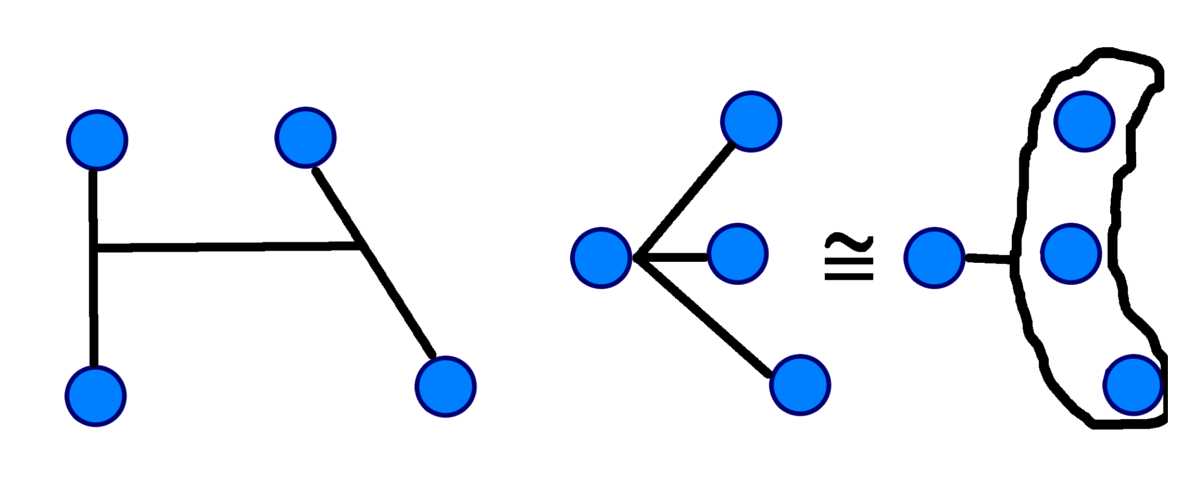
\includegraphics[scale=0.3]{Images/exampleadj.png}
    \end{center}
    \caption{Метавершинная и метареберная смежности}
    \label{fig:imgMVAMEA}

\end{figure}

Далее на основании определения изоморфизма графовых структур сформулированы и доказаны соответствия наиболее популярных классов графов и метаграфов.

% В каком виде и какая смежность взята

\textbf{Теорема 1.} Для любого графа $G$ существует как минимум один изоморфный метаграф $MG$, построенный с помощью отображения, которое любому элементу ставит множество из одного элемента $\varphi(v) = \{v\}$ и сохраняет отношение смежности. Назовем данный изоморфизм тривиальным.
\\$\Box$\\
$G=\langle V,E \rangle=\Big \langle\{v_1,v_2,...,v_n \},\big\langle ..., \{ v_i, v_j \}, ... \big\rangle \Big\rangle$, $ MG=\langle V,ME \rangle. \text{ } G \cong MG $\\$ \text{при } \varphi(v) = \{v\}$. $\text{Тогда 	} ME=\big\langle ..., \{ \varphi(v_i), \varphi(v_j) \}, ... \big\rangle$
\vspace{-0.6cm}
\begin{flushright}
$\blacksquare$
\end{flushright}
\vspace{-0.6cm}

\textbf{Следствие.} Любому метаграфу, метаребра которого не содержат множеств более чем из одного элемента, можно сопоставить изоморфный ему граф с обратным тривиальным изоморфизмом $\varphi^{-1}(\{ v \}) = v$.
\\$\Box$\\
 $MG=\langle V,ME \rangle = \Big\langle \{ v_1,...,v_n \},\big\langle ..., \langle \{v_i\}, \{v_j\} \rangle, ... \big\rangle \Big \rangle, \text{ }G = \langle V,E \rangle. \text{ } G \cong MG $\\$ \text{при } \varphi^{-1}(\{ v \}) = v$. $G=\Big \langle\{v_1,v_2...v_n \},\big\langle ..., \{ \varphi^{-1}(\{v_i\}), \varphi^{-1}(\{v_j\}) \}, ... \big\rangle \Big\rangle=$\\$\Big \langle\{v_1,v_2...v_n \},\big\langle ..., \langle v_i, v_j \rangle, ... \big\rangle \Big\rangle$.
 \vspace{-0.6cm}
\begin{flushright}
$\blacksquare$
\end{flushright}
\vspace{-0.6cm}

\textbf{Теорема 2.} Пусть $I\langle V,E\rangle$ -- матрица инцидентности графа $G$ и $I\langle V, ME \rangle$ -- матрица инцидентности метаграфа $MG$, тогда при тривиальном изоморфизме они тождественно равны.
\\$\Box$\\
$|ME|=|E|$, так как $\forall e \in E \text{ } \exists! \text{ }me \in ME \text{ такое, что при } e_k = \{v_i,v_j\} \text{, } me_k = \langle \{v_i\},\{v_j\} \rangle$. $\text{Следовательно, } I_{ij}\langle V, E \rangle = 1 \Leftrightarrow I_{ij}\langle V, ME \rangle=1 \text{ по определению.}$ В общем виде для идентификации метавершин необходимо одной из метавершин ставить единицу с противоположным знаком.
 \vspace{-0.6cm}
\begin{flushright}
$\blacksquare$
\end{flushright}
\vspace{-0.6cm}

\textbf{Теорема 3.} Для любого полного графа $K_{n}$ существует изоморфизм, помимо тривиального, при котором количество метаребер изоморфного ему метаграфа $MK_{n}$ будет равно $n-1$. 
\\$\Box$\\ Метаребра строятся рекурсивно. Для этого занумеруем в любой последовательности вершины и, начиная с первой, будем соединять с вершинами, у которых номер больше. В итоге получим $n-1$ метаребро.
Определение для полного графа: 
$$\forall v_{i}\in V \text{ } \forall v_{j} \in V: i \neq j \text{ } \psi(v_{i}, v_{j}) = 1,$$
нетривиальный полный метаграф:$$\forall v_{i} \in V \text{ } \exists \bar{V}: (\forall j>i \text{  } v_{j} \in \bar{V}) \text{ }\psi(\langle v_i \rangle, \langle v_j \rangle) = 1,$$
где $\psi$ - функция смежности.


$G=\langle V,E \rangle=\Big \langle\{v_1,v_2,...,v_n \},\big\langle \langle v_1, v_2 \rangle, \langle v_1, v_3 \rangle,...,\langle v_1, v_n \rangle,...,\langle v_{n-1}, v_{n} \rangle \big\rangle \Big\rangle\text{,}$\\$  G \cong MG\text{ при } \varphi(\langle v_i,v_{i+1}\rangle,...,\langle v_i,v_n \rangle) = \langle \{v_i\}, \{v_{i+1}, ..., v_{n}\} \rangle. \text{ Тогда } MG=\Big \langle V,\big\langle \langle \{v_1\}, \{v_2,v_3,..., v_n\} \rangle,...,\langle \{v_{n-1}\}, \{v_{n}\} \rangle \big\rangle \Big\rangle$.
\vspace{-0.6cm}
\begin{flushright}
$\blacksquare$
\end{flushright}
\vspace{-0.6cm}

\textbf{Теорема 4.} Пусть $I\langle V,E \rangle$ и $I\langle V, ME\rangle$ матрицы инцидентности полного графа $K_n$ и изоморфного ему по теореме 3 метаграфа. Тогда $I\langle V, ME\rangle$ -- нижнетреугольная матрица, состоящая из единиц, с главной диагональю из минус единиц.\\
$\Box$ \begin{center}
 $I\langle V,E \rangle$ = \begin{tabular}{c|ccccccc|}
&$e_1$ &$ e_2$ & $...$ & $e_{n-1}$ & $e_n$ & ... & $e_m$ \\ \hline
$v_1$ & 1 & 1 & ... & 1 & 0 & ... & 0 \\ 
$v_2$ & 1 & 0 & ... & 0 & 1 & ... & 0 \\ 
$v_3$ & 0 & 1 & ... & 0 & 1 & ... & 0 \\ 
... & ... & ... & ... & ... & ... & ... & ... \\ 
$v_{n-1} $&0 & 0 & ... & 0 & 0 & ... & 1 \\ 
$v_{n}$ & 0 & 0 & ... & 0 & 1 & ... & 1 \\ 
\end{tabular},
\end{center}
где $n = |V|$, а $m = \dfrac{n\cdot(n-1)}{2}$. 
\begin{center}
$I\langle V, ME\rangle$ = \begin{tabular}{c|cccccc|}
&$e_1$ &$ e_2$ & $e_3$ & $e_4$ & ... & $e_m$ \\ \hline
$v_1$ & -1 & 0 & 0 &0& ... & 0 \\ 
$v_2$ & 1 & -1 & 0 &0& ... & 0 \\ 
$v_3$ & 1 & 1 & -1 &0& ... & 0 \\ 
... & ... & ... &...& ... & ... & ... \\ 
$v_{n-1} $&1 & 1 & 1& 1 & ... & -1 \\ 
$v_{n}$ & 1 & 1 & 1&1 & ... & 1 \\ 
\end{tabular},
\end{center}
где $n = |V|$, а $m=n-1$. 
\vspace{-0.6cm}
\begin{flushright}
$\blacksquare$
\end{flushright}
\vspace{-0.6cm}

\textbf{Теорема 5.} Для любого полного $2$-дольного графа $K_{p,q}$ существует изоморфный метаграф (кроме тривиального), причем множество метаребер будет состоять из одного метаребра $\langle V_1, V_2\rangle$, такого что $V_1$ и $V_2$ будут совпадать с долями.
\\$\Box$ Перенумеруем вершины так, чтобы первые $p$ были в одной доле, следующие $q$ в другой.
\\$G=\langle V,E \rangle=\Big \langle\{v_1,v_2...v_n \},\big\langle ..., \{ v_i, v_j \},...\big\rangle \Big\rangle$, где $i, j$ такие, что

\begin{equation*}
 \begin{cases}
  p < j \leq p+q = n, & 0 < i \leq p,\\
  0 < j \leq p, & p < i \leq p+q=n,
 \end{cases}
\end{equation*}	
\\$\text{тогда обозначим } V_1 = \{v_1,v_2, ..., v_p\} \text{ и } V_2 = \{v_{p+1}, ..., v_{q+p=n}\}.$
$\text G \cong MG= \langle V, ME \rangle \text{ при } $$\varphi(E) =ME = \big \langle \langle V_1,V_2 \rangle \big \rangle$. Поскольку любой элемент первой доли смежен с любым элементом второй доли, то метаграф $MG\cong G$.
$\blacksquare$


\textbf{Теорема 6.} Полному $n$-дольному графу соответствует изоморфный метаграф (кроме тривиального), причем множество метаребер будет состоять из метаребер, составленных как при построении полного графа $K_n$, но вместо элементов будут входить множества $V_1,...,V_n$, которые представляют собой непосредственно доли.
 \\$\Box$ Аналогично двудольному случаю введем множества, которые будут обозначать множества элементов конкретных долей: $V_1,V_2,...,V_n$. По определению нам нужно, чтобы каждый элемент был смежен со всеми элементами других долей, а также не смежен с элементами из своей доли. Тогда задача сводится к построению $n$-полного графа (Теорема 3) с $n-1$ метаребром, но вместо элементов в $n$-полном графе будут выступать доли $V_1,...,V_n$. 
 $\blacksquare$


\textbf{Теорема 7.} Для любого цикла $C_{n}$ не существует нетривиального изоморфного ему метацикла $MC_{n}$. Исключение составляют $C_3$ (совпадает с $K_3$), $C_4$ (совпадает с $K_{2,2}$).

$\Box$ В цикле у каждой вершины не может быть больше чем две смежные вершины, а при введении метаребра, отличного от тривиального, будет получаться больше двух смежных вершин. Исключения составляет $C_3$ (совпадает с $K_3$), $C_4$ (совпадает с $K_{2,2}$), что согласуется с теоремами 3 и 5. 
\vspace{-0.6cm}
\begin{flushright}
$\blacksquare$
\end{flushright}
\vspace{-0.6cm}

\subsection{Развитие матричного представления обобщенных графовых структур}
Графовые структуры удобно представлять с помощью матриц. Основными матрицами для описания графовых структур являются матрицы инцидентности ($I$), смежности ($A$), валентности ($D$) и лапласиан ($L$). Более того, они связаны следующим равенством: 
\begin{equation} \label{eq:rel1}
	L=I\times I^{\tau} = D \pm A.
\end{equation}

Для итергиперграфов, наиболее общего класса графовых структур, в \cite{BluminIterGG} вводится показатель итерации как инвариант графовых структур, и описывается расширенный класс графовых моделей на основе понятия итерированных булеанов множеств, с помощью которых указывается связь для матриц инцидентности. Для метаграфов данная связь будет выглядеть следующим образом: 
\begin{equation} \label{eq:rel2}
I(V, ME) = I(V, MV) \cdot I(MV, ME).
\end{equation}
Кроме этих представлений, наподобие тому, как в \cite{JoslynN17} гиперграф был представлен с помощью графа инцидентности, так можно представить и метаграф. Для любого метаграфа $MG=\langle V, MV, ME \rangle$ существует граф инцидентности $KMG\langle V,E\rangle$, подобно графу Кёнига для графа и гиперграфа. Поскольку в метаграфе невозможно говорить о смежности вершин в терминах графов и гиперграфов, а именно из-за наличия второй смежности, вводится вспомогательное множество метавершин $MV$, и граф инцидентности получается трехдольным, где первая доля -- это вершины, вторая -- это метавершины, третья -- это метаребра. Таким образом, этот граф Кёнига охватывает все две смежности метаграфа. Между вершинами и метавершинами -- отношение принадлежности (аналогично инцидентности в гиперграфе) для кластеризации вершин по признаку совместной смежности, а между метавершинами и метаребрами -- отношение инцидентности (аналогично инцидентности в графе). Причем справедливо равенство для матричных представлений:
$$L_{KMG}\langle V,E \rangle = I_{KMG}\langle V,E \rangle \cdot (I_{KMG}\langle V,E \rangle)^\tau= $$
$$
\left(
\begin{array}{c|c|c}
 \begin{array}{ccc}
  l_{1,1} & ...& 0\\
  \vdots& \ddots &\vdots \\
  0&... & \ddots
 \end{array}
  & I(V, MV) & 0 \\
\hline
(I(V,MV))^\tau & \begin{array}{ccc}
  \ddots & ...& 0\\
  \vdots& \ddots &\vdots \\
  0&... & \ddots
 \end{array} & I(MV, ME) \\
\hline
0 & (I(MV,ME))^\tau & \begin{array}{ccc}
  \ddots & ...& 0\\
  \vdots& \ddots &\vdots \\
  0&... & l_{|V|+|MV|+|ME|,|V|+|MV|+|ME|}
 \end{array}
\end{array}
\right),$$ где $l_{i,i}=\sum\limits_{k=1}^{|V+E|}|l_{i,k}|=\sum\limits_{k=1}^{|V+E|}|l_{k,i}|.$


В конечном итоге получается, что для однозначной записи метаграфа может быть использована одна из приведенных выше матричных структур (или две в случае матрицы валентности), причем при представлении метаграфа графом, а именно графом инцидентности, матричные представления базируются на исходных, в частности, лапласиан графа инцидентности поблочно состоит из матриц инцидентности $I(V,MV), I(MV, ME)$ соответствующего метаграфа. Все представления графовых структур отражают сущность одного объекта, но с разных сторон, и используются в зависимости от постановки задачи. Матричное представление графовых структур, которое, к слову, сейчас редко используется в программном обеспечении, также обладает рядом преимуществ, в числе которых возможность использования архитектуры параллельных и распределенных вычислений для вычислений на уровне примитивов, строгая алгебраическая формализация, применимость средств линейной алгебры и основанных на ней методов прикладной математики, а также вариативность представления в зависимости от условий задачи. 

Критерий изоморфизма в подразделе 1.2.1. был сформулирован, основываясь на понятии смежности, а вследствие и теоремы о изоморфизме некоторых классов графов и метаграфов также основывались на понятии смежности; стоит отметить, что это было сделано исключительно для компактности и простоты изложения в теоретико-множественном виде и является одним из возможных вариантов. Ключевую же роль играют матрицы инцидентности и основанные на них фундаментальные соотношения матричной теории графоструктурного моделирования, которые связывают между собой все указанные выше матрицы. Поэтому теоремы о изоморфизме, где присутствовали матричные представления, были сформулированы именно с матрицами инцидентности. Матрицы смежности и валентности и лапласианы строятся по одним и тем же правилам для всех графовых структур, в отличие от матриц инцидентности. Так, например, при переходе к оргиперграфам для задания ориентации используются комплексные корни из единицы в качестве элементов матрицы инцидентности, а в случае метаграфа, как было видно из теорем 2 и 4, для идентификации метавершин в качестве элементов матрицы используется $\pm 1$. 

\subsection{Алгоритм преобразования графа в метаграф}
Нами был разработан алгоритм, преобразующий матрицу инцидентности графа в матрицу инцидентности изоморфного ему метаграфа.
\begin{enumerate}
	\item Запишем граф в виде матрицы инцидентности $I(V,E)$.
	\item Если матрица $I(V,E)=\mathbb{O}$, то алгоритм завершен.
	\item Находим строку в $I(V,E)$ с максимальным количеством единиц (вершину с максимальной валентностью).
	\item Добавляем метаребро в $I(V,ME)$, содержащее в одной метавершине эту вершину, а в другой метавершине вершины, смежные с данной.
	\item Обнуляем в $I(V,ME)$ найденную строку и столбцы, значения которых в этой строке равны единице.
	\item Переходим к пункту 2.
\end{enumerate}

\subsection{Применение графоструктурного моделирования в задачах обработки и анализа больших данных}

Применение графоструктурного подхода к решению задач больших данных можно условно разделить на два вида -- это непосредственно моделирование исходных данных графовыми структурами и моделирование информационных систем (ИС), с помощью которых решаются эти задачи. 

Для того, чтобы перевести исходные данные в графоструктурный вид, необходимо, чтобы данные были представимы графами в контексте решаемой задачи. Важно заметить, что любой объект может быть сведен к составляющим и описан с некоторой точностью графовыми структурами, но это описание должно иметь прямую связь с постановкой задачи. Наиболее продуктивен этот подход для задач с разнообразными сетями, где исходные данные -- это и есть структура, описываемая графами; например, социальные сети, веб-графы, биологические сети, сети транспортных дорог и т.д. Стоит также отметить, что эти сети являются очень большими и сложно структурированными, поэтому вопрос о применении обобщенных графовых структур более чем актуален для данного рода объектов. В качестве обоснования можно выделить ряд преимуществ: сокращение размерности исходных данных без потери информации, снижение сложности интерпретации промежуточных и конечных результатов за счет повышения уровня абстракции рассматриваемого объекта, а также возможность новой постановки задачи с вытекающей возможностью применения других методов; например, задача, известная как задача китайского почтальона \cite{chinaPostman}. Суть класса таких задач состоит в принадлежности дуг к определенным множествам, не обязательно дизъюнктным, где нужно найти кратчайший путь через дуги всех этих множеств. В классической постановке задача формализуется через ряд ограничений, недавние результаты по одной из таких задач можно посмотреть в \cite{metroParis}. Если рассматривать задачу в терминах метаграфов, то вместо введения ограничений и отображения множества ребер в другое множество (обычно множество цветов) можно определить для каждого множества (цвета) метавершину, и тогда решением будет кратчайший путь через все метавершины. 

Большинство сложных задач интеллектуального анализа данных ставится таким образом, что адекватное решение становится возможным исключительно при использовании нескольких информационных интеллектуальных систем (ИИС), работающих как одно целое, так называемых гибридных интеллектуальных систем (ГИИС) \cite{BluminPrinkovTend, ChernenkiiPI, ChernenkiiNRP, ChernenkiiNI}. Функционирование таких ГИИС возможно посредством последовательного применения алгоритмов к исходным данным, такие системы моделируются с помощью графов, иными словами, это тогда, когда ГИИС имеет линейное графоструктурное представление, где вершины последовательно связаны между собой, при этом возможны петли и циклы. Для представления более сложных интеллектуальных систем, например, когда одна ИИС может модифицировать другую в зависимости от результатов обработки исходных данных в текущий момент времени или когда ГИИС может дифференцироваться на другие ГИИС, которые, в свою очередь, также имеют произвольную структуру, необходимо использовать более развитые графовые структуры -- такие, как гиперграфы, метаграфы. Это также важно, когда нужно параллельно применить несколько алгоритмов из одного класса и корректно совместить результаты в один.

На сегодняшний день в различных прикладных областях применения ИИС и ГИИС свою эффективность показал подход к ремоделированию графовых структур гиперграфовыми, которое можно осуществить как было указано в подразделе 1.2.3. Основная проблема такого подхода -- это то, что для такого ремоделирования необходимо находить максимально полные подграфы в графе, впоследствии заменяя их гиперребрами, тем самым сокращая размерность и структурируя исходные данные, а эта задача является вычислительно неполиномиальной, в отличие от задачи кластеризации ребер в метаребра, которая носит более эвристический характер и позволяет добиться результатов не хуже, чем гиперграфовый подход, причем наряду с этим вычислительно менее затратна. Алгоритм для преобразования графа в метаграф был описан в подразделе 1.2.3.

Программную реализацию простейших видов ГИИС можно найти в библиотеке машинного обучения sklearn. Pipeline
-- это линейная структура ГИИС, в которой последовательно выполняются статистические алгоритмы. Это обеспечивает автоматизацию решения задачи, где вместо того, чтобы вручную выполнять каждый из алгоритмов на тренировочном и тестовом наборах данных, используется декларативный интерфейс. В качестве применяемых алгоритмов могут выступать как методы извлечения, преобразования, нормализации данных, так непосредственно и сама модель предиктора. Эта структура (рисунок \ref{iisigiis}) не описывает ГИИС, принципиально отличимую от ИИС, в отличие от структуры FeatureUnions. FeatureUnions позволяет применять алгоритмы параллельно к одному набору данных и объединять результаты, что очень полезно, например, при преобразовании текста в численный вид, где в связи с тем, что после применения одного из алгоритмов исходные данные будут переведены в численную форму, информация, присутствующая в априорном виде набора данных, станет недоступной. Таким образом, комбинируя эти две структуры, можно моделировать разичные варианты ГИИС. Справа на рисунке \ref{iisigiis} показана ГИИС структуры FeatureUnions, предназначенная для классификации предложений на естественном языке по некоторым признакам. Исходя из вышесказанного, разработка структур моделей представления более сложных ИИС и ГИИС обобщенными графовыми структурами является весьма актуальной. 

Для того, чтобы оперировать текстом, необходимо его представить в числовом виде. Иначе говоря, нужно применить лексический анализатор, переводящий произвольный текст $x$ в численный вид $x'$, к набору исходных данных 
$$x' = g(x), g:\mathbb{L} \to \mathbb{R}^{n_1},$$
 где $\mathbb{L}$ -- это множество допустимых синтаксических конструкций естественного языка. Также для извлечения, преобразования и нормализации данных используются следующие виды отображений-трансформаторов 
 $$x_2' = h(x_1'), h: \mathbb{R}^{n_1} \to \mathbb{R}^{n_2}.$$

При последовательном применении $g_1$, а затем $h_1$ получается суперпозиция $h_1(g_1(x))$. Тогда следует принять тот факт, что  $h_1:\mathbb{R}^{n_1} \to \mathbb{R}^{n_2}$, а следовательно при последовательном применении мы можем применить только один лексический анализатор. Процесс предварительной обработки данных можно записать как 
$$h_n(...(h_1(g_1(x)))), g_1 : \mathbb{L} \to \mathbb{R}^{n_1}, h_i:\mathbb{R}^{n_{i}} \to \mathbb{R}^{n_{i+1}}. $$
Такое использование полностью покрывается графовыми моделями, но не является единственно возможным. Для параллельной обработки данных необходимо использовать метаграфовую структуру ГИИС. Тогда 
$$x_g' = Gx =
\left(
\begin{array}{c}
g_1 \\
g_2\\
\vdots \\
g_{n-1}\\ 
g_{n}
\end{array}
\right)^{\tau}
\left(
\begin{array}{ccccc}
x & 0 & ... &  0 & 0 \\
0 & x & ... & 0 & 0 \\
\vdots & \vdots & \vdots & \vdots & \vdots \\
0 & 0 & ... & x & 0 \\
0 & 0 & ... & 0 & x
\end{array}
\right)  = 
\left(
\begin{array}{c}
g_1(x) \\
g_2(x)\\
\vdots \\
g_{n-1}(x)\\ 
g_n(x)
\end{array}
\right)^{\tau}.
$$ 
После чего получится разреженная матрица, которую неободимо преобразовать в векторную форму
$$x_{g}' = m_g(x'), m_g : \mathbb{R}^{n_1 \times n} \to \mathbb{R}^{n'},$$
к которой можно применить отображения-трансформаторы либо последовательно
$$h_n(...(h_1(g_1(x_{g})))), g_1 : \mathbb{L} \to \mathbb{R}^{n_1}, h_i:\mathbb{R}^{n_{i}} \to \mathbb{R}^{n_{i+1}},$$
либо параллельно
$$x'_h = H m_g (Gx) =
\left(
\begin{array}{c}
h_1 \\
h_2\\
\vdots \\
h_{n-1}\\ 
h_{n}
\end{array}
\right)^{\tau}
\cdot
m_g
\left(\left(
\begin{array}{c}
g_1 \\
g_2\\
\vdots \\
g_{n-1}\\ 
g_{n}
\end{array}
\right)^{\tau}
\cdot\left(
\begin{array}{ccccc}
x & 0 & ... &  0 & 0 \\
0 & x & ... & 0 & 0 \\
\vdots & \vdots & \vdots & \vdots & \vdots \\
0 & 0 & ... & x & 0 \\
0 & 0 & ... & 0 & x
\end{array}
\right) \right)  = 
\left(
\begin{array}{c}
h_1(x'_g) \\
h_2(x'_g)\\
\vdots \\
h_{n-1}(x'_g)\\ 
h_n(x'_g)
\end{array}
\right)^{\tau}.
$$ 
В случае параллельного применения отображений-трансформаторов, следует также применить агрегирующую функцию, как и в случае с синтаксическими анализаторами:

$$x_{h}' = m_h(x'), m_h : \mathbb{R}^{n_2 \times n} \to \mathbb{R}^{n'}.$$
Важно заметить, что и к $x'_h$, и к $x'_g$ можно неограниченное число раз применять как последовательное, так и параллельное преобразование отображениями-трансформаторами.

\section{Разработка программного обеспечения для статистической обработки больших данных проката}

\newpage
\section{Апробация разработанных методов и программного обеспечения для обработки больших данных по холодной прокатке с целью выявления чаттера}
